\documentclass[12pt,a4paper]{article}

\usepackage[T1]{fontenc}
\usepackage[utf8]{inputenc}
\usepackage[brazil]{babel}
\usepackage{graphicx}
\usepackage{geometry}
\usepackage{listings}
\usepackage{listingsutf8}
\usepackage{xcolor}
\usepackage{setspace}
\usepackage{float}
\usepackage{tikz}
\usepackage{tabularx}

\usetikzlibrary{positioning, shapes.geometric}
\onehalfspacing
\geometry{margin=2.5cm}

\lstset{
    language=SQL,
    basicstyle=\ttfamily\small,
    keywordstyle=\color{blue},
    commentstyle=\color{gray},
    stringstyle=\color{red},
    breaklines=true,
    showstringspaces=false
}

\newcommand{\montarinicio}[3]{
    % =========================
    % CAPA
    % =========================
    \begin{titlepage}
        \centering

        {\large Faculdade Anhanguera}\\[0.5cm]
        {\large Tecnólogo em DevOps}\\[3cm]

        {\Large \textbf{#1}}\\[2cm]

        {\large Gabriel Blank Stift Mousquer}\\[1cm]

        {\large Ivoti/RS}\\
        {\large 2026}

    \end{titlepage}

    % =========================
    % FOLHA DE ROSTO
    % =========================
    \begin{titlepage}
        \centering

        {\large Faculdade Anhanguera}\\[0.5cm]
        {\large Tecnólogo em DevOps}\\[2cm]

        {\Large \textbf{#1}}\\[1.5cm]

        \begin{flushright}
            Trabalho apresentado à disciplina de \\
            \textbf{#2} \\
            Professor: #3 \\
        \end{flushright}

        \vfill

        {\large Gabriel Blank Stift Mousquer}\\
        Matrícula: 2024201126\\

        \vfill

        {\large Ivoti/RS}\\
        {\large 2026}

    \end{titlepage}

    % =========================
    % SEÇÃO: TOC
    % =========================
    \tableofcontents
    \newpage
}


\begin{document}

\montarinicio
    {TRABALHANDO COM UMA TABELA NO BANCO DE DADOS}
    {Programação e Desenvolvimento de Banco de Dados}
    {Thaysla Fernanda Da Cruz Cardoso}

% =========================
% SEÇÃO: INTRODUÇÃO
% =========================

\section{Introdução}

O presente trabalho tem como objetivo demonstrar a utilização de comandos da linguagem SQL no contexto de manipulação de bancos de dados relacionais, conforme proposto na atividade prática. Em particular, busca-se compreender e aplicar instruções básicas como \texttt{SELECT}, \texttt{FROM} e \texttt{WHERE}, bem como comandos de definição de dados (DDL) para a criação de tabelas.

Além disso, são abordadas operações de inserção, consulta e manipulação de dados em um banco de dados MySQL, incluindo o uso de cláusulas como \texttt{GROUP BY} e \texttt{ORDER BY}, bem como operações com strings por meio do operador \texttt{LIKE} e funções de agregação, como \texttt{SUM}.

As atividades foram realizadas em um ambiente baseado no sistema operacional \textit{Ubuntu 24.04.4 LTS}, utilizando o sistema gerenciador de banco de dados \textit{MySQL}, versão 8.0.45, acessado por meio de sua interface de linha de comando (CLI).

Para a execução dos comandos, foi utilizado um usuário específico, denominado \texttt{aula1}, criado exclusivamente para a realização das operações propostas. O acesso ao banco de dados foi efetuado via terminal, utilizando o comando \texttt{mysql -u aula1 -p}.

A partir desse ambiente, foram executadas as etapas previstas no exercício, incluindo a criação do banco de dados, definição de tabelas, inserção de dados e realização de consultas, conforme descrito nas seções seguintes.

\section{Desenvolvimento}

Inicialmente, procedeu-se à criação do banco de dados denominado
\textit{empresa}, conforme ilustrado na Figura~\ref{fig:criar-db}.

\begin{figure}[H]
    \centering
    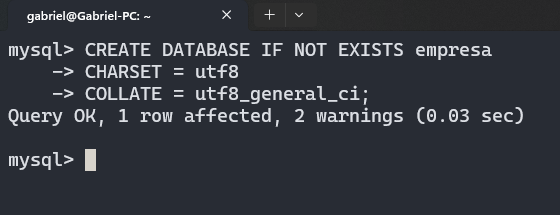
\includegraphics[width=0.8\textwidth]{./static/1-criar-db.png}
    \caption{Criação do banco de dados}
    \label{fig:criar-db}
\end{figure}

Na sequência, foi utilizado o comando \texttt{USE} com o objetivo de selecionar o banco de dados previamente criado, estabelecendo-o como contexto ativo para a execução das demais instruções, conforme apresentado na Figura~\ref{fig:use-db}.

\begin{figure}[H]
    \centering
    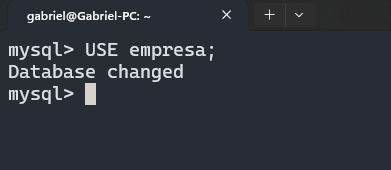
\includegraphics[width=0.8\textwidth]{./static/2-use-db.png}
    \caption{Seleção do banco de dados ativo}
    \label{fig:use-db}
\end{figure}

Posteriormente, realizou-se a criação da tabela denominada \textit{funcionarios}, contemplando as colunas especificadas no enunciado do exercício, a saber: \textit{id}, \textit{nome}, \textit{departamento}, \textit{salario} e \textit{data\_admissao}. A execução dessa etapa pode ser observada na Figura~\ref{fig:criar-tabela}.

\begin{figure}[H]
    \centering
    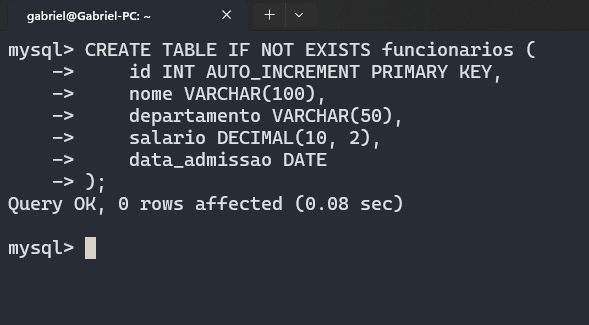
\includegraphics[width=0.8\textwidth]{./static/3-criar-tabela.png}
    \caption{Criação da tabela funcionarios}
    \label{fig:criar-tabela}
\end{figure}

Com a estrutura da tabela definida, procedeu-se à inserção de dados de exemplo, com o intuito de possibilitar a realização de consultas significativas. Foram incluídos registros referentes a, no mínimo, cinco funcionários, distribuídos em diferentes departamentos e faixas salariais, conforme ilustrado na Figura~\ref{fig:inserir-dados}.

\begin{figure}[H]
    \centering
    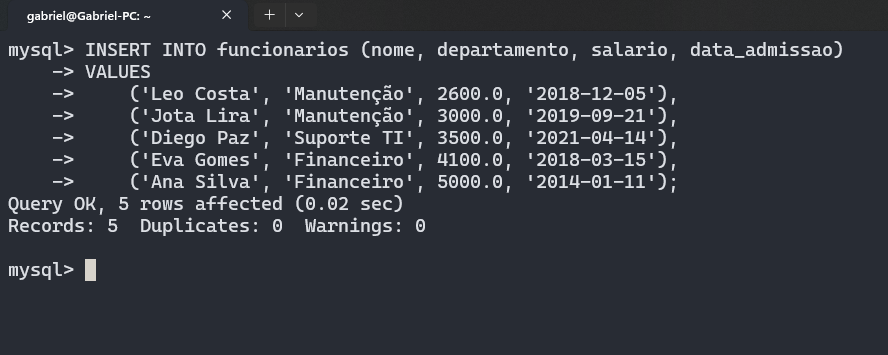
\includegraphics[width=0.8\textwidth]{./static/4-inserir-dados.png}
    \caption{Inserção de dados na tabela funcionarios}
    \label{fig:inserir-dados}
\end{figure}

A partir dos dados inseridos, foram realizadas consultas com o objetivo de explorar as informações armazenadas. Inicialmente, executou-se uma consulta para listar todos os funcionários pertencentes a um departamento específico, conforme apresentado na Figura~\ref{fig:consulta-1}.

\begin{figure}[H]
    \centering
    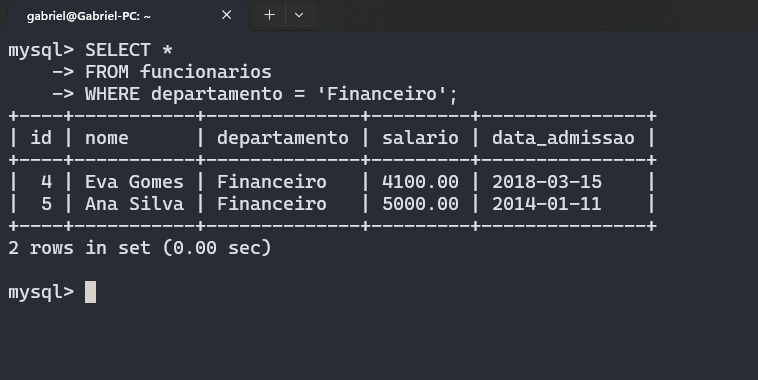
\includegraphics[width=0.8\textwidth]{./static/consulta-1.png}
    \caption{Consulta de funcionários por departamento}
    \label{fig:consulta-1}
\end{figure}

Em seguida, foi realizada uma consulta para exibir o nome e o departamento de todos os funcionários, aplicando-se uma transformação para que os resultados fossem apresentados em letras maiúsculas, conforme demonstrado na Figura~\ref{fig:consulta-2}.

\begin{figure}[H]
    \centering
    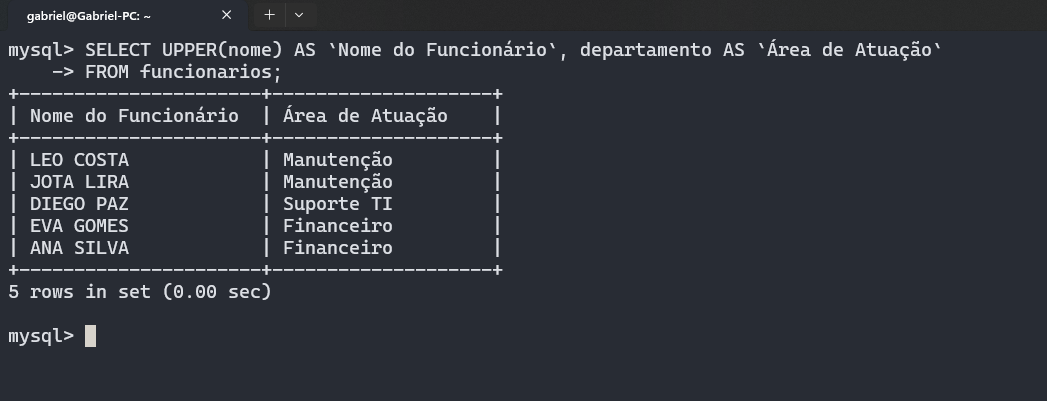
\includegraphics[width=0.8\textwidth]{./static/consulta-2.png}
    \caption{Consulta com formatação em letras maiúsculas}
    \label{fig:consulta-2}
\end{figure}

Posteriormente, efetuou-se uma consulta com o objetivo de calcular o total de salários por departamento, com os resultados organizados em ordem decrescente, conforme ilustrado na Figura~\ref{fig:consulta-3}.

\begin{figure}[H]
    \centering
    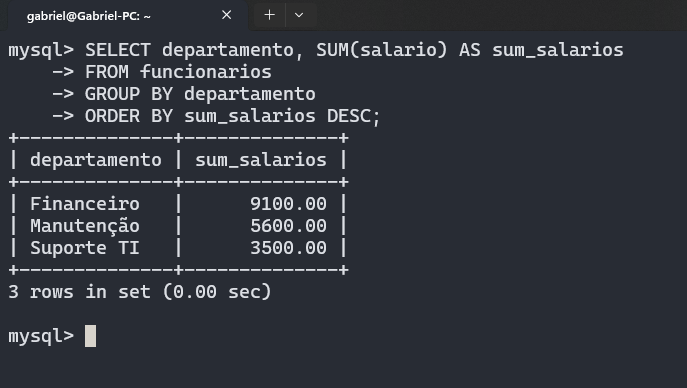
\includegraphics[width=0.8\textwidth]{./static/consulta-3.png}
    \caption{Total de salários por departamento}
    \label{fig:consulta-3}
\end{figure}

Por fim, foi realizada uma consulta para identificar os funcionários cujos nomes se iniciam com a letra “A”, conforme apresentado na Figura~\ref{fig:consulta-4}.

\begin{figure}[H]
    \centering
    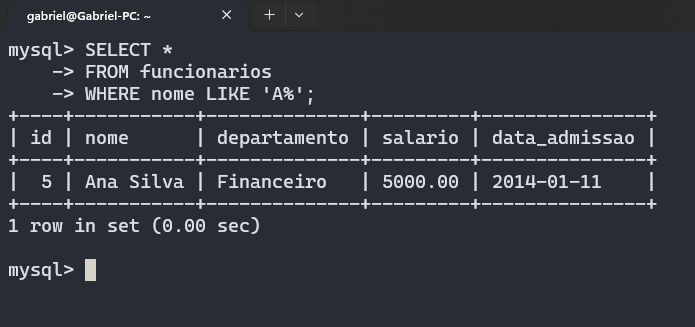
\includegraphics[width=0.8\textwidth]{./static/consulta-4.png}
    \caption{Consulta de funcionários com nomes iniciados pela letra A}
    \label{fig:consulta-4}
\end{figure}

% =========================
% SEÇÃO: CONCLUSÃO
% =========================
\section{Conclusão}

A realização da atividade permitiu aplicar, na prática, comandos básicos de SQL para criação de tabelas, inserção de dados e execução de consultas.

Durante o desenvolvimento, ficou evidente que consultas como \texttt{SELECT} com filtros (\texttt{WHERE}) são essenciais para recuperar informações específicas, enquanto recursos como \texttt{GROUP BY} e funções de agregação, como \texttt{SUM}, permitem analisar os dados de forma mais consolidada. Já o uso de operadores como \texttt{LIKE} facilita buscas por padrões em textos.

O domínio dessas consultas é relevante em contextos práticos, pois sistemas reais frequentemente exigem a extração de informações específicas a partir de grandes volumes de dados. Consultas com filtros, ordenação e agrupamento são utilizadas, por exemplo, para gerar relatórios, analisar dados operacionais e apoiar decisões com base nas informações armazenadas.

Dessa forma, a atividade contribuiu para compreender não apenas a sintaxe dos comandos, mas também sua aplicação na obtenção de informações úteis em cenários que se aproximam do uso real de bancos de dados.

% =========================
% SEÇÃO: APÊNDICE
% =========================
\section{Apêndice}

\subsection{Script SQL completo}

\lstinputlisting[
    caption={Script SQL completo},
    label={lst:sql},
    inputencoding=utf8/latin1,
    basicstyle=\ttfamily\scriptsize
]{./static/script.sql}

\end{document}
